%% ----------------------------------------------------------------
%% Final_Report.tex
%% ---------------------------------------------------------------- 
%%Preamble
\documentclass{IEEEtran}			 % Use the GDP Report Style
%\graphicspath{{../Figures/}}   				% Location of your graphics files

\usepackage[english]{babel}
\usepackage{graphicx}
\usepackage{subfigure}

\usepackage{natbib}           					 % Use Natbib style for the refs.
\usepackage{listings} 							%Package to include source code.
\usepackage{booktabs}
\usepackage{pdflscape}       	% Enables the use of landscape orientation of pages
\usepackage{longtable}        % Enables a table to cut across more than one page
\usepackage{tabu}         		% Used together with longtable for the above purpose
\usepackage{multirow}					% Used for the multi column testing table (for power)
\usepackage{bigstrut}					% Used for the multi column testing table (for power)
%\usepackage{appendix}			% To use \appendixpage to add Appendix Chapter
\usepackage{color}				% listings colour
\usepackage{float}
\usepackage{fixltx2e}
\usepackage{hyperref}
\usepackage{mathtools}


\usepackage{tabularx}
\usepackage{dblfloatfix}% http://ctan.org/pkg/dblfloatfix
\usepackage{lipsum}% http://ctan.org/pkg/lipsum
%\newcommand{\plus}{\raisebox{.4\height}{\scalebox{.6}{+}}}	% Used for the small + and - signs in the power testing table
%\newcommand{\minus}{\raisebox{.4\height}{\scalebox{.8}{-}}} % Used for the small + and - signs in the power testing table

%\lstset{language=C}   					%Set source code language to 'c'
%\usepackage[inline]{enumitem} 			%In line lists
%\usepackage{paralist}
%\usepackage{tensor}			% Enables writing super- and sub- scripts on left hand side

%\definecolor{dkgreen}{rgb}{0,0.6,0}
%\definecolor{gray}{rgb}{0.5,0.5,0.5}
%\definecolor{mauve}{rgb}{0.58,0,0.82}
%\definecolor{lightblue}{rgb}{0.80,0.95,1.0}



\begin{document}
\title      {Custom IC Design Assignment 1}
\author    {

\texorpdfstring {\href{mailto:xb1g10@ecs.soton.ac.uk}{Xuan Ban}} {Xuan Ban}  
\texorpdfstring {\href{mailto:xb1g10@ecs.soton.ac.uk}{xb1g10}} {xb1g10} \\ 
    {\href{mailto:xb1g10@ecs.soton.ac.uk}{Yang Huihuang}} 
	\texorpdfstring  {\href{mailto:hy9g10@ecs.soton.ac.uk}{hy9g10}} {hy9g10} \\   
    {\href{mailto:xb1g10@ecs.soton.ac.uk}{Dedic Charlie}} 
	\texorpdfstring  {\href{mailto:cd2g11@ecs.soton.ac.uk}{cd2g10}} {cd2g11} {23922516} \\
    {\href{mailto:xb1g10@ecs.soton.ac.uk}{Wang Chu}}             
	\texorpdfstring  {\href{mailto:cd2g10@ecs.soton.ac.uk}{cw9g10}} {cw9g10} \\
	Group 1
            }
\date       {\today}

\maketitle

\begin{abstract}
Abstract goes here. Use this latex template as our report template.
\end{abstract}



%% ----------------------------------------------------------------
%% ----------------------------------------------------------------
%% Introduction.tex
%% ---------------------------------------------------------------- 


%\chapter[Introduction]{Introduction} \label{Chapter:Introduction}
\section{Introduction} \label{Section:Introduction}
In this exercise, the final goal is to design, test and demonstrate an 8-bits affine transformation implementation of picoMIPS on an Altera FPGA development system. A simple affine transform\cite{affine} can be defined as such: 
\begin{align}
	{x2 \choose y2} = A \times {x1 \choose y1} + B
\end{align}

The specific A and B datasets were chosen for the demonstration in this exercise, which are:
\begin{align}
 A = \begin{bmatrix}
       0.75 & 0.5           \\[0.3em]
       -0.5 & 0.75          \\[0.3em]
     \end{bmatrix}   		
%\end{align}	
%\begin{align}	
 B= \begin{bmatrix}
        20          \\[0.3em]
       -20          \\[0.3em]
     \end{bmatrix}
\end{align}

In the picoMIPS program design, the six transformation constants must be included as immediate literals. The switches SW0-7 on the FPGA development system are required for Pixel coordinates input. The LEDs LED0-7 are assigned to display the transformation result. Switch SW8 controls the handshaking functionality to complete the transform sequence, as described below. The switch SW9 is used as an active low reset.
\begin{table}[H]
%
\centering % used for centering table
\begin{tabular}{ll}
\hline
1 & When SW8 is on read the coordinate x1 from SW{[}7:0{]}, otherwise wait. \\ 
2 & Wait until SW8 is off                                                   \\
3 & When SW8 is on read the coordinate y1 from SW{[}7:0{]}, otherwise wait  \\
4 & Wait until SW8 is off                                                   \\
5 & Execute the affine transformation for x2 and display it on LED{[}7:0{]}        \\
6 & Wait until SW8 is on                                                    \\
7 & Execute the affine transformation for y2 and display it on LED{[}7:0{]}                                              \\
8 & Wait until SW8 is off. If so go back to step 1                          \\ \hline

\end{tabular}
\caption{Instruction Set} % title of Table
\end{table}
During the preparation, the picoMIPS architecture and SystemVerilog code examples of each picoMIPS block that are provided by ELEC6016 lecture slides were well studied and tested in the Modelsim. During the first stage of the design, a set of Systemverilog codes were developed based on the preparation and a successful working design was achieved to fulfil the basic requirement of the exercise. Separate testbenchs for the individual modules and the top-level design were also implemented and simulated in Modelsim to verify the correct functionality of the design. The input and output 8‐bit data were assigned to the designated ports. All modules were successfully synthesised and programed into the FPGA Development System. \\\\
At the second stage of the development, the goal was focused on optimizing the original design to reduce the cost figure as much as possible. The cost figure is defined as:\\\\
                    Cost = number of Logic Elements used + 30 x Kbits of RAM used\\\\
The optimization includes the usage of the synchronous RAM and simplification of the instruction set and other picoMIPS modules. As the result, the cost figure was successfully reduced from 132 to 76.\\\\
This report is split into two major sections. Section 2-4 will describe the original design and section 6 will discuss the AE0 synthesis and optimized design in detail. The cost figure discussion for each design will be included in conclusion section.



\section{NAND logic gate}
In this exercise the design of the NAND gate was expected to have minimum area while to have high fanout output(fanout =8). In order to find the delay time between input and output of the NAND gate, the Elmore Delay model~\cite{elmore1948transient} was used in the design.\\
\subsection{Design and Optimization}
As shown in the Figure~\ref{fig:nand}, NAND gate is constructed by two parallel connected PMOS transistors and two serial connected NMOS transistors. 

\begin{figure*}[ht]
\centering
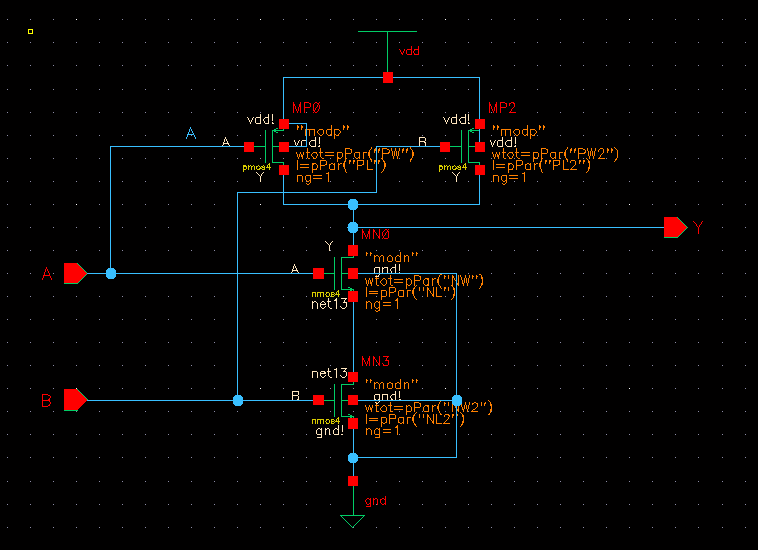
\includegraphics[width = 0.7\textwidth]{Figures/nand}
\caption{NAND gate schematic}
\label {fig:nand}
\end{figure*}

Although transistors have complicate current-voltage behaviour, turned on transistors can be assumed as resistors, a chain of transistors can be represented as an RC ladder, as shown in Figure~\ref{fig:elmore}. Therefore the Elmore delay model can estimate the delay of this RC ladder in terms of the path resistance and capacitance of a node on the ladder and the supply:

\begin{align}
	{t\textsubscript{pd} = \sum_{\substack{i}} R\substack{n-i}C\substack{i}}
\end{align}

\begin{figure}[H]
		\centering
		%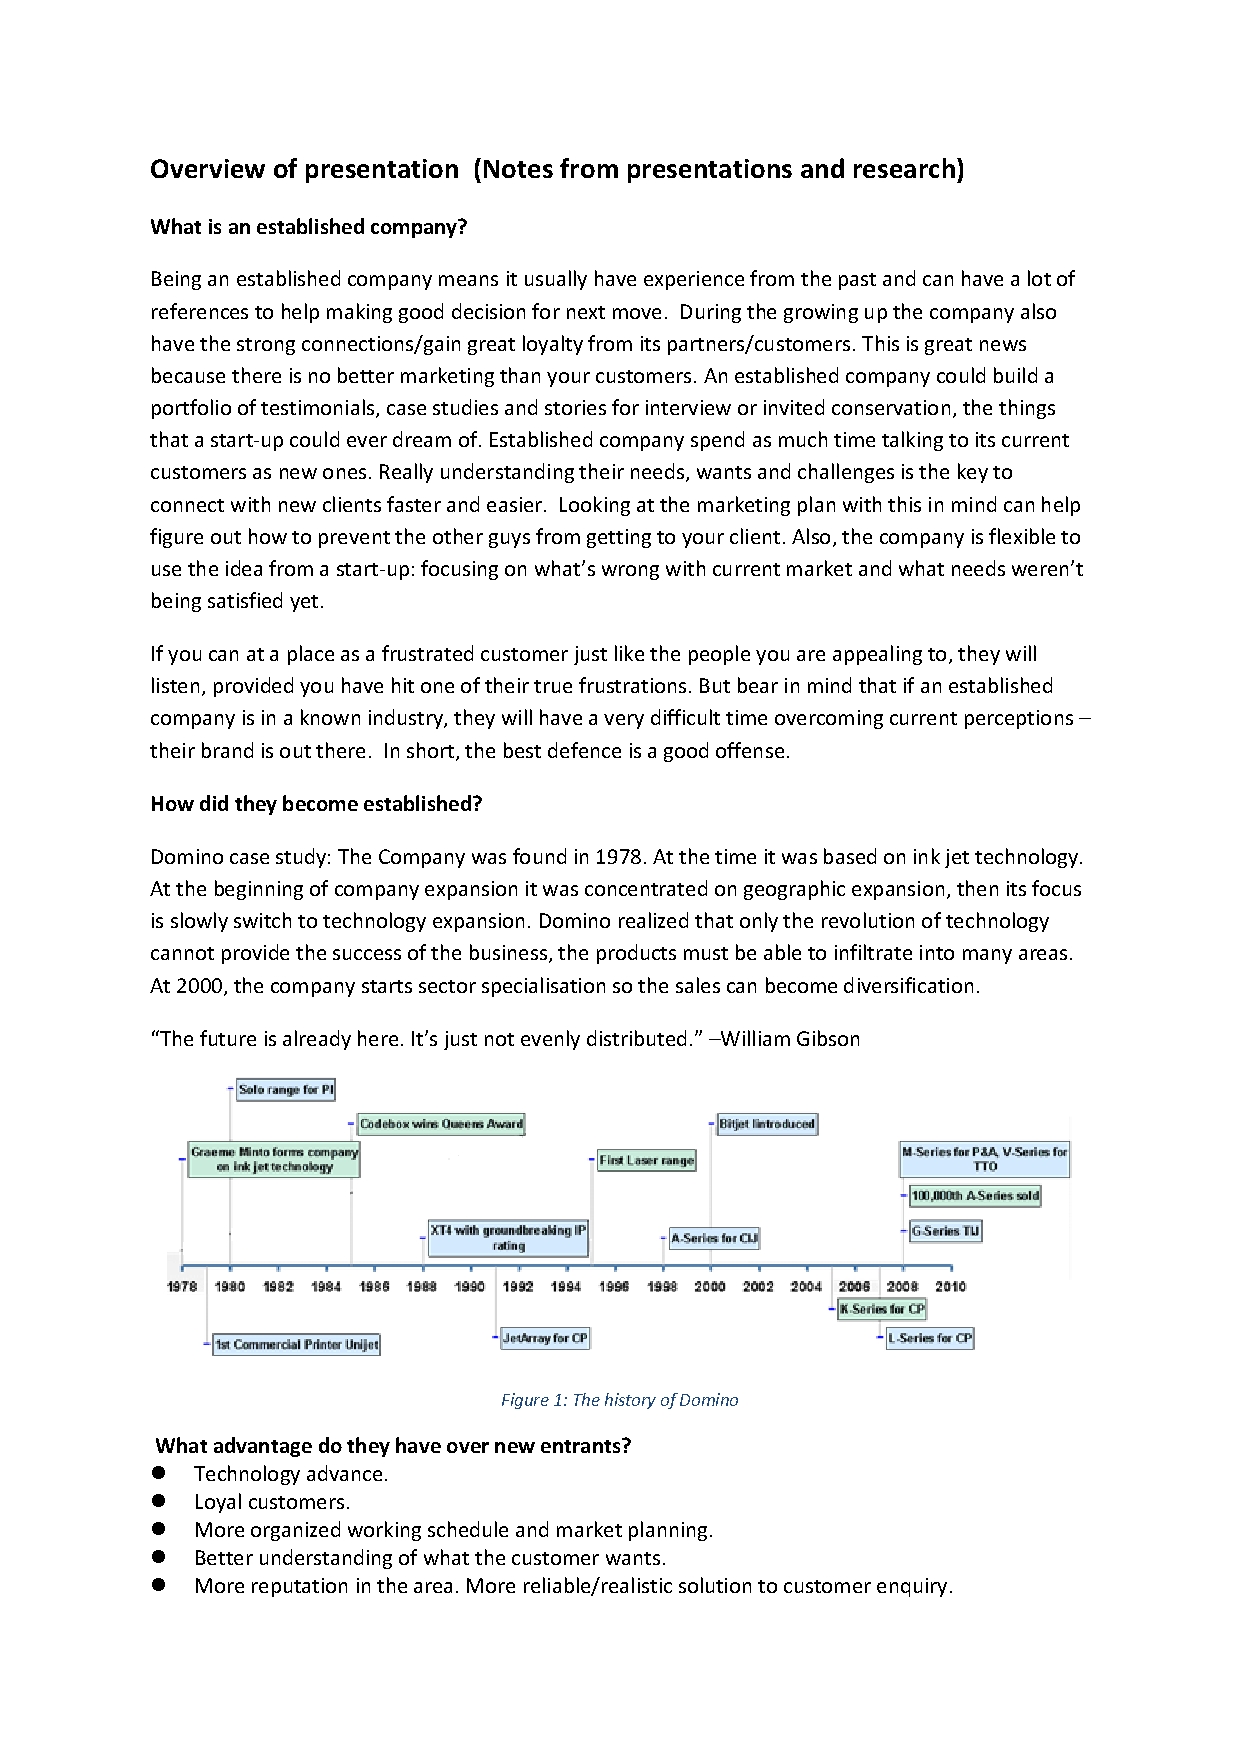
\includegraphics[width = 0.9\textwidth]{Figures/Overview_of_presentations}
		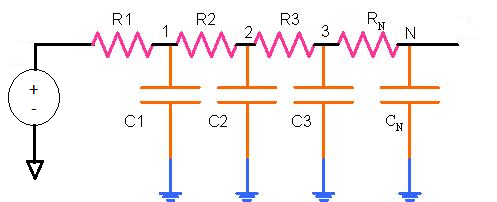
\includegraphics[width = 0.45\textwidth]{Figures/elmoredelaymodel}		
		\caption{Simple Elmore delay model}
		\label {fig:elmore}
\end{figure}
Therefore it is possible to use this method as the reference to calculate the width of logic gate, since the propagation delay is dependent to it and the capacitance of the load. \\
Typically in the logic gate, for parallel connected  transistors, the total resistance is lower when they are all on. In many gates, the worst-case delay is usually because only on the parallel transistor is on~\cite{[2]}. So when applying the Elmore delay model in the NAND design, one of input is connected to vdd while the other one is connected in the path, as shown in Figure~\ref{fig:nandtest}.
\begin{figure}[H]
		\centering
		%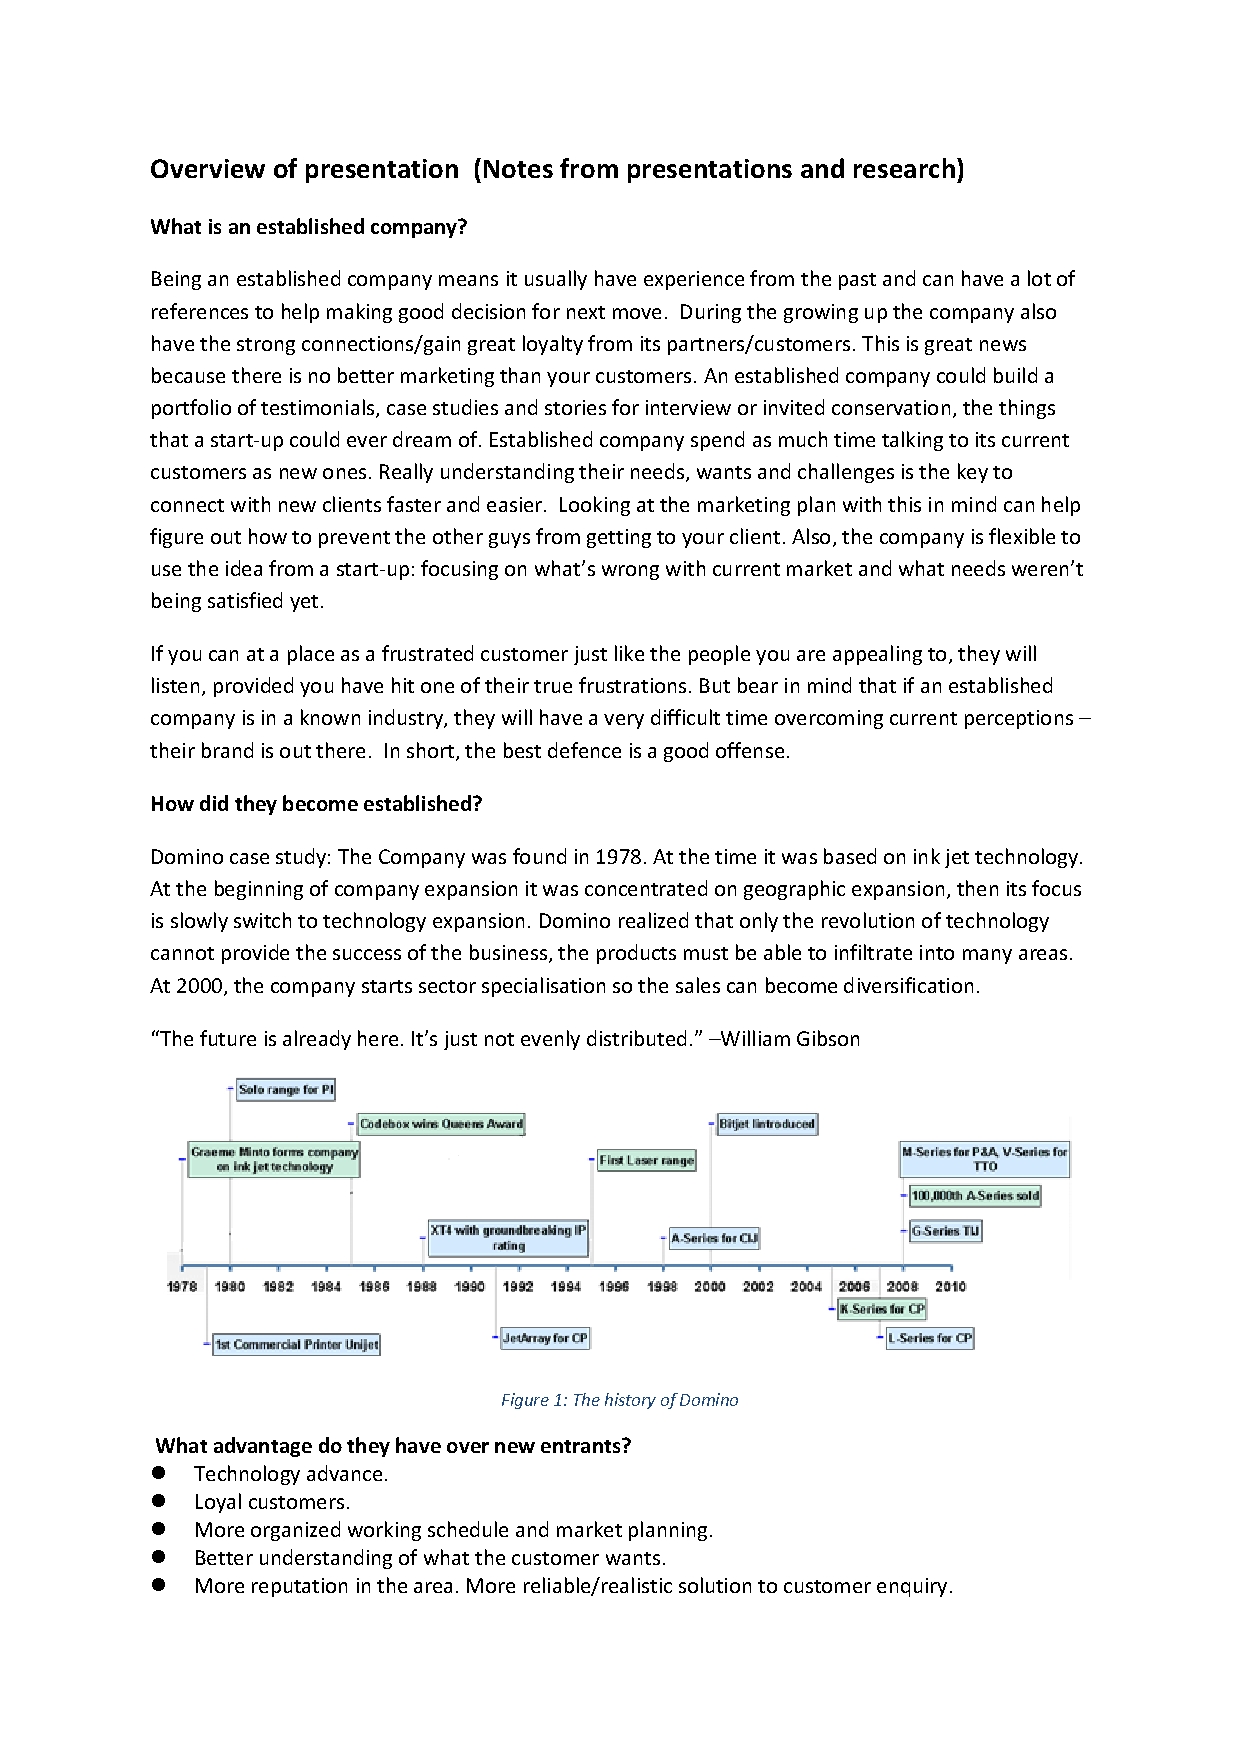
\includegraphics[width = 0.9\textwidth]{Figures/Overview_of_presentations}
		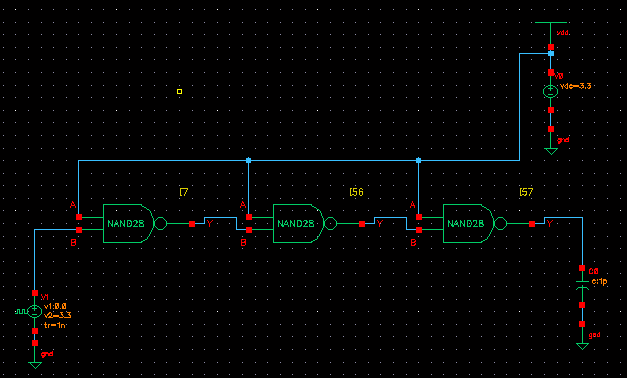
\includegraphics[width = 0.5\textwidth]{Figures/nandtest}		
		\caption{NAND Elmore delay model}
		\label {fig:nandtest}
\end{figure}

While deceasing the width of NMOS and increasing the width of PMOS, the propagation delays, which is the maximum time from input to output crossing 50\%, of the rising edge and falling edge are also changing. When the certain ratio between the width of PMOS and NMOS is reached, the propagation delay between rising edge and falling edge of logic gate will become similar. In another word, the signal slope at the output of logic gate will become quite identical to the input, only with an amount of delay.\\
In the design, the ratio between PMOS and NMOS is 2.3, as found in the Figure~\ref{fig:NANDratio}.
\begin{figure}[hf]
		\centering
		%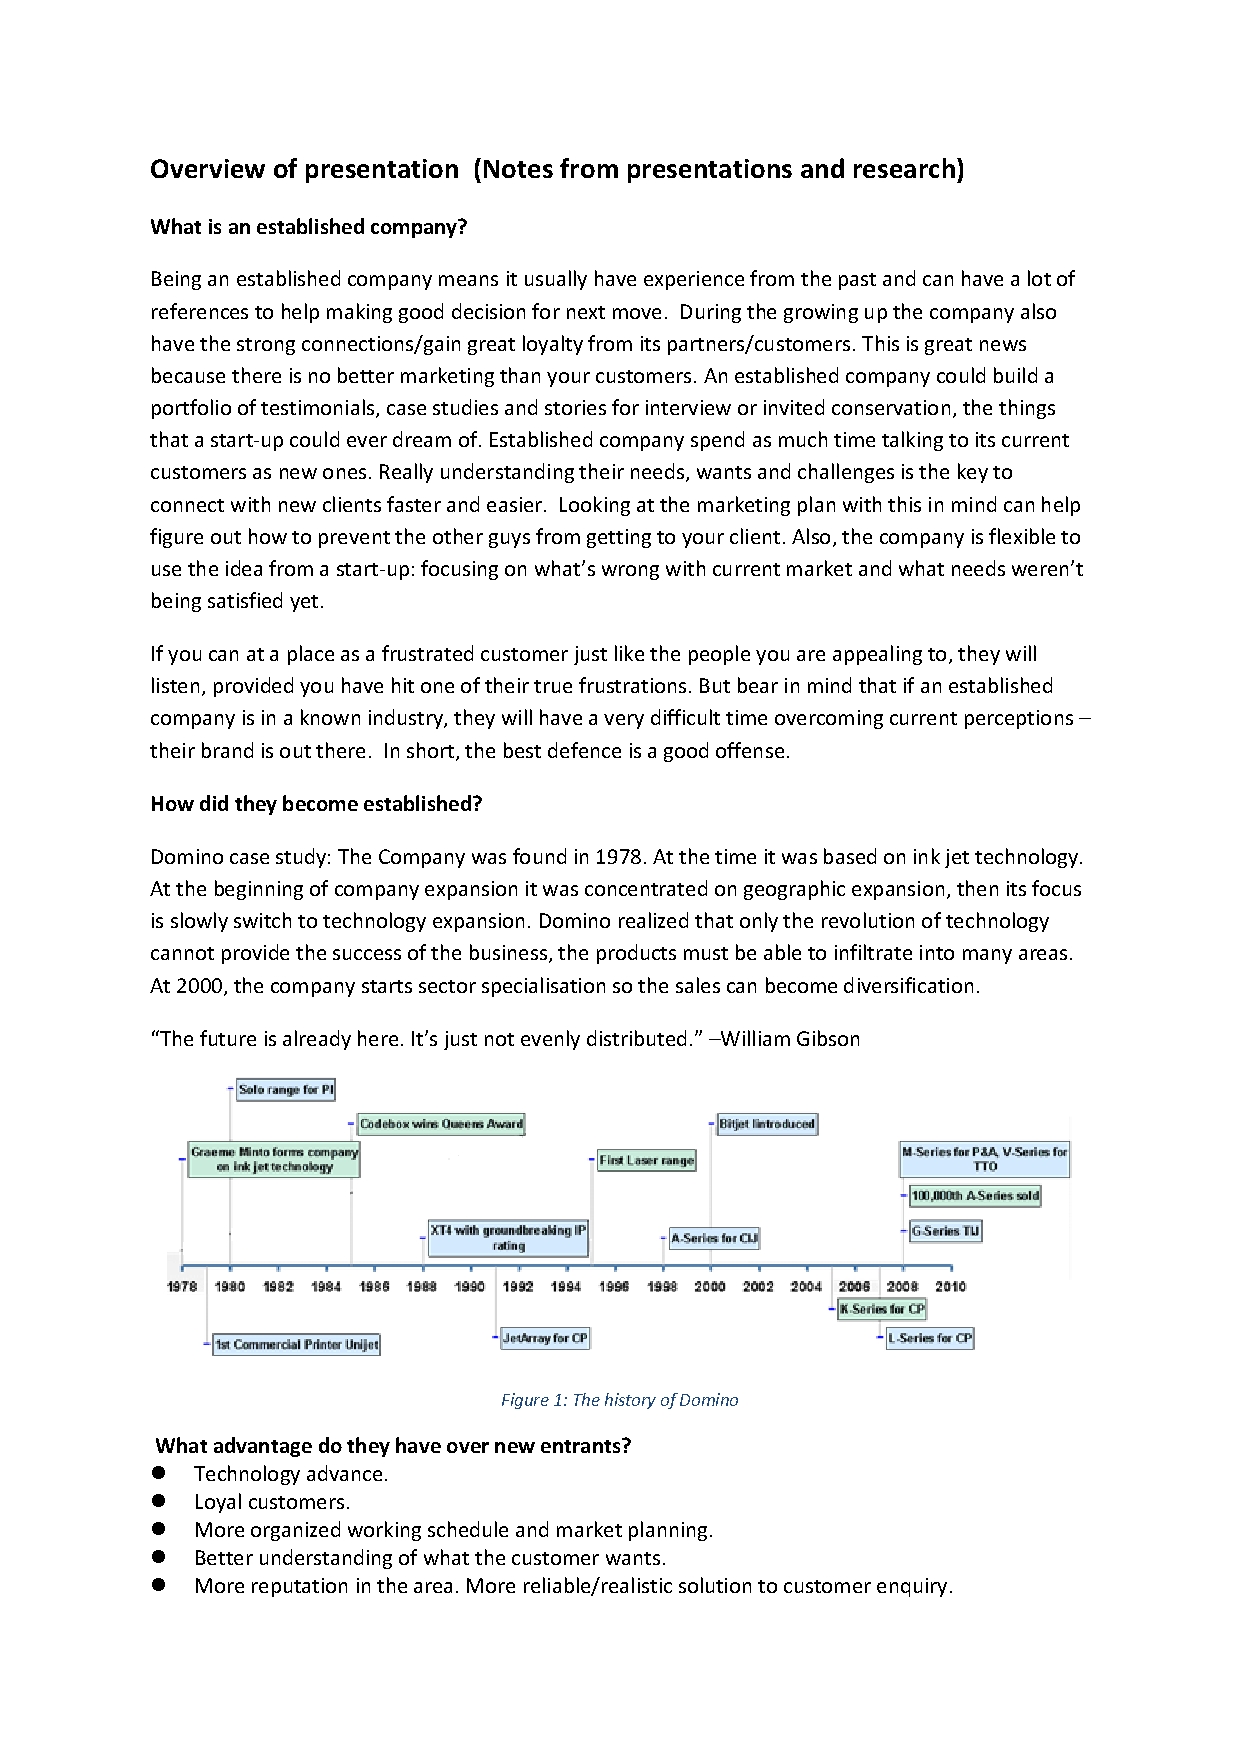
\includegraphics[width = 0.9\textwidth]{Figures/Overview_of_presentations}
		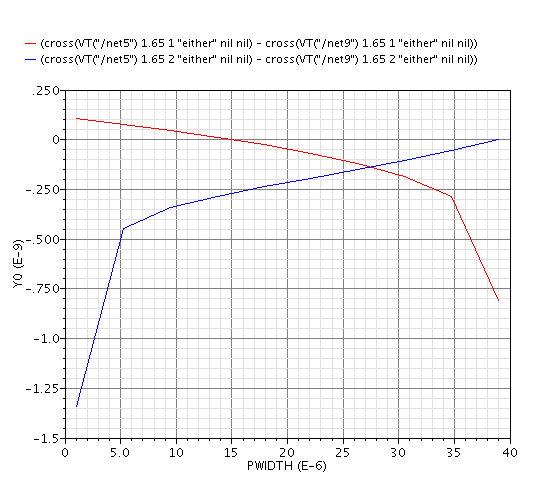
\includegraphics[width = 0.5\textwidth]{Figures/NANDratio}		
		\caption{Ratio of width of PMOS and NMOS in NAND gate}
		\label {fig:NANDratio}
\end{figure}

If a gate can drive n copies of itself, then it is said to have a fanout or electrical effort of n. When multiple gates are chain connected together to form a multi-stage logic network, Since the ratio between size of PMOS and NMOS is confirmed, the next procedure is determining the actual size of transistors in the NAND gate.

\chapter{Design and Optimisation} 


\section{NAND}

\section{NOR2}

\section{XOR2}

\section{DFF}
The design goal for the DFF was high speed. Initially it was designed using a standard circuit composed of NAND gates. However then the option of Transmission gates was considered and found to be superior. Using transmission gates a master slave style flip plot was produced as shown in figure \ref{fig:DFFSchem}. A ratio between PMOS and NMOS of 3 was chosen as it is the integer ratio which produced the best results for rise and fall time matching. As 0.35$\mu$ is the length set by the technology used the only parameter used is NWIDTH for each gate as PWIDTH is simply 3 times that.

\begin{figure}[h]  
\centering
   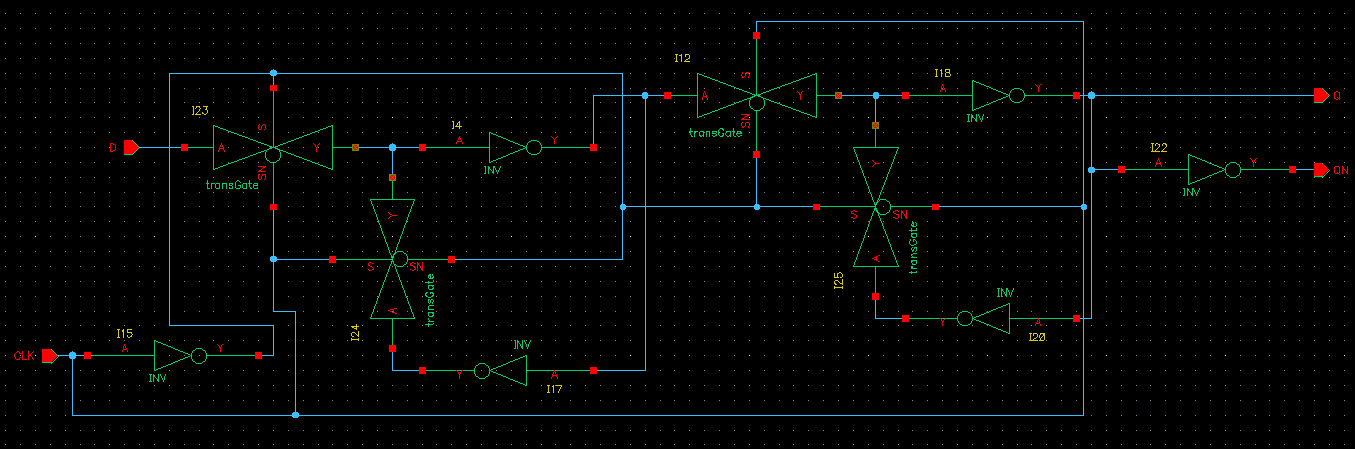
\includegraphics[width=0.45\textwidth]{Figures/DFFSchem.png}
\caption{DFF Schematic.}
\label {fig:DFFSchem}
\end{figure}

In terms of transistor sizes the Transmission gate and the Inverters were considered as separate parameters although there was only one size for each family This may have been a bad decision in terms of the inverter creating CLKN as it has to drive 4 components where as the maximum of any other gate was only 2, However in this situation it was not much of a problem as the relatively large transistor sizes chosen to deliver high speed negated much of this effect.

By using the rise times, as shown in figure \ref{fig:DDFNW}, among other metrics when measured in the test circuit Values for NMOS and PMOS widths were chosen based on giving maximum performance. These turned out to be a 11$\mu$m for the transmission gate and 17.5 $\mu$m for the inverter. This is quite large but as the only restriction on the design is that it must be high speed regardless of area.

\begin{figure}[h]
\centering
\subfigure[Inverter N Width]{
  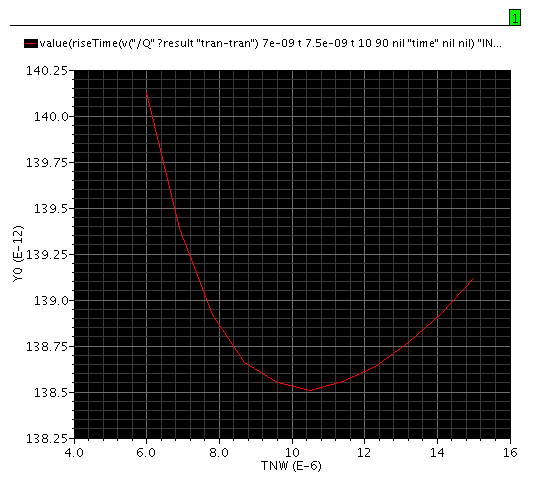
\includegraphics[width=.225\textwidth]{Figures/DFF1fFLoadTNW.png}
  \label{fig:DFFINW}}
\subfigure[Transmission gate N Width]{
  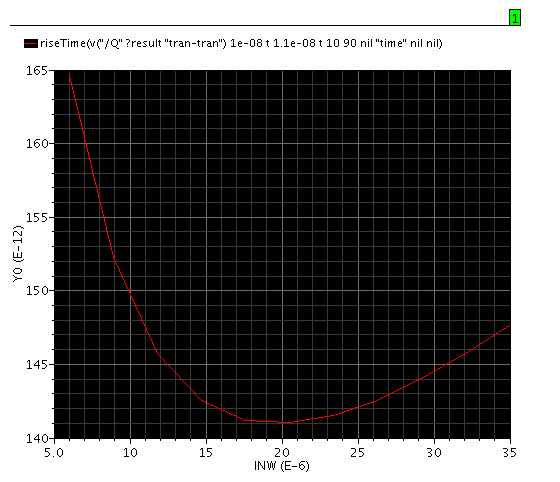
\includegraphics[width=.225\textwidth]{Figures/DFF1fFLoadINW.png}
  \label{fig:DDFTNW}}
\caption{Transistor size effect on rise time.}
\label{fig:DDFNW}
\end{figure}

One point of note is that the QN output is created via a separate inverter rather than taking the signal from either side of the left most transmission gate. This was because large capacitive loads on QN caused incorrect circuit behaviour as this effected the transition time across the transmission gate which incorrect circuit behaviour on extreme loads where the slave circuit wouldn't latch new master value.

\begin{figure}[h]  
\centering
   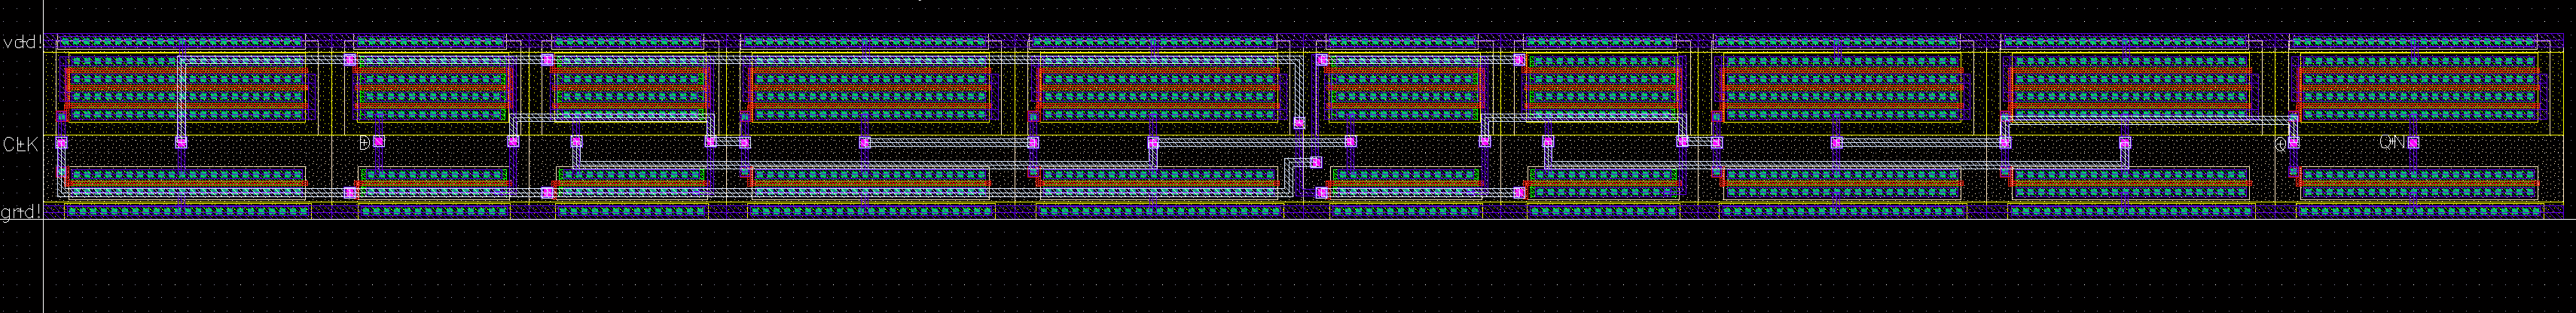
\includegraphics[width=0.45\textwidth]{Figures/DFFLayout.png}
\caption{DFF Layout.}
\label {fig:DFFLayout}
\end{figure}

Due to the large transistor size layout was not particularly difficult as there was a lot of space for gate interconnects. When laying out the gates were placed in an order such as to minimise local process variations however with such large gates this is not particularly effective. A future layout revision could increase robustness by splitting the transistors into 2 or 3 smaller transistors of equal total size and interleaving them.

\section{Duel Edge Triggered Flip Flop}

The Dual Edge Triggered Flip Flop (DETFF) was designed using transmission gates as this allows the design to contain a minimum of 20 transistors (18 if there is no requirement for QN). Figure \ref{fig:DETFFSchem} shows the schematic produced. A ratio between PMOS and NMOS of 3 was chosen as it is the integer ratio which produced the best results for rise and fall time matching. As 0.35$\mu$ is the length set by the technology used the only parameter used is NWIDTH for each gate as PWIDTH is 3 times that.

\begin{figure}[h]  
\centering
   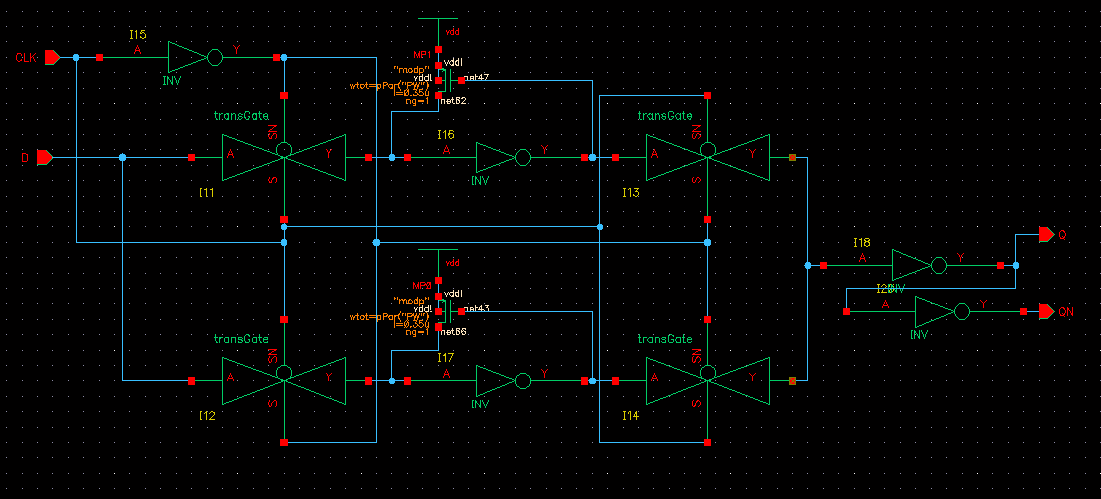
\includegraphics[width=0.45\textwidth]{Figures/DETFFSchem.png}
\caption{DETFF Schematic.}
\label {fig:DETFFSchem}
\end{figure}

The size of the gates where considered in terms of Transmission gates NMOS Width, Inverters NMOS Width and the 2 PMOS pull up transistors width. These parameters were brought to minimum  values of 1.2$\mu$m 2$\mu$m and 4$\mu$m (Trans NW,Inv NW,Pwidth respectively) before correct operation ceased. However these values were found to be to small for effective layout without enough space for interconnects and routing to fit due to DRC constraints, they also gave speed performance deemed unacceptable. The sizes were increased until sensible routing and speed was achieved  at values of 2.4$\mu$m 3.2$\mu$m and 4.7$\mu$m (Trans NW,Inv NW,Pwidth respectively).

\begin{figure}[h]  
\centering
   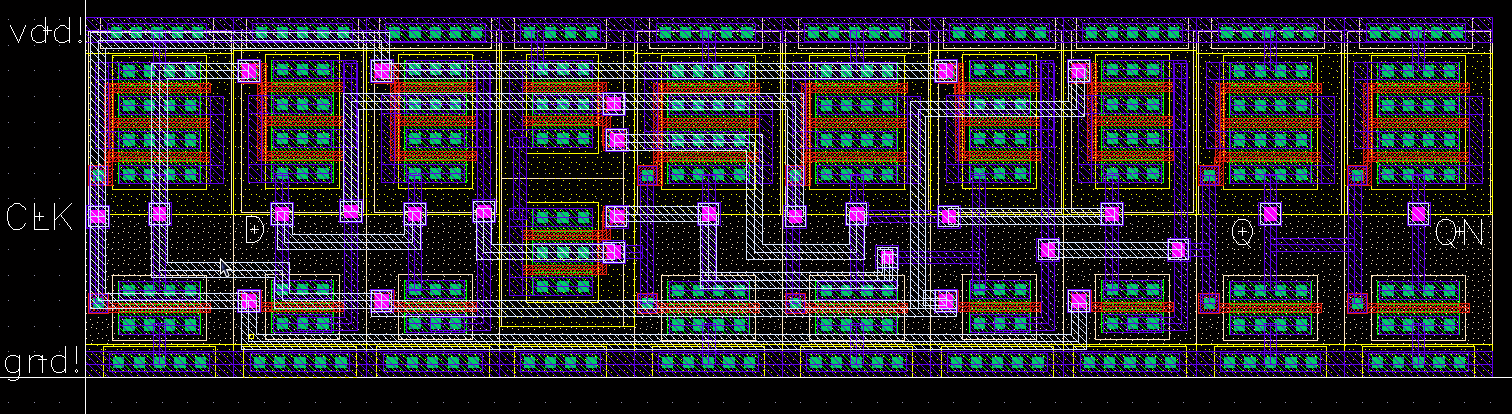
\includegraphics[width=0.45\textwidth]{Figures/DETFFLayout.png}
\caption{DETFF Layout.}
\label {fig:DETFFLayout}
\end{figure}

Figure \ref{fig:DETFFLayout} shows the final layout of the DETFF its easily visible that this is towards the limit of gate size for the given layout in particular in crowded areas such as the between gates 6 and 7. The option of using MET3 in this area was considered but it was not specified this layer was available for use also as a consideration to real world manufacture having to add another metal layer because of a single gate when a 2 layer design is possible would not be viable.

The layout of the design initial versions of the Transmission and inverter were lain out  at the minimum possible width and copied to populate the design and as interconnects were placed some of them had the wells expanded to allow for interconnect spacing.The pull-up PMOS are stacked vertically so as to not waste horizontal space as the rail distance is fixed meaning total area is effected by the width of the entire gate.

\section{C Element}

\section{Dual Rail AND}
The design goal for the Dual Rail AND was small area. The design was chosen based on its simplicity and the fact that the C-Element had the same goal of small area. This fact allowed us to simply reuse the C-Element with fixed parameters and reuse its layout saving substantial amounts of work in layout. there is a disparity between the Required fan-outs however as the fanout of the c-element is two and the AND has a fanout of one meaning the extra area gained is not too great.

\begin{figure}[h]  
\centering
   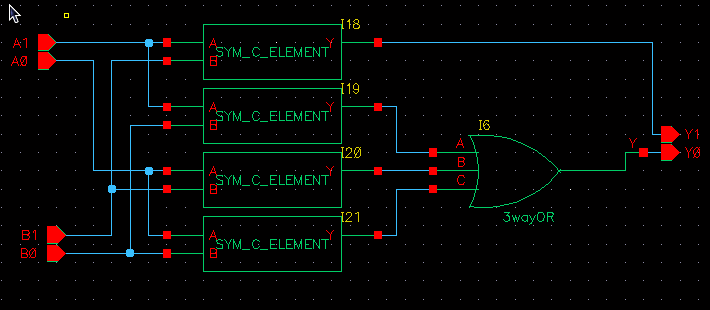
\includegraphics[width=0.45\textwidth]{Figures/DualRailANDSchem.png}
\caption{Dual Rail AND Schematic.}
\label {fig:DualRailANDSchem}
\end{figure}

The only element in this design that required optimisation in design was the 3 input OR gate. This was constructed from a 3 input NOR gate and an inverter on the output. The PMOS and NMOS ratio was set at 3 and the characteristics matched to that of the output of the C-element meaning there should be minimum disparity between the Y0 and Y1 signals. The Nwidth was finalised at 4$\mu$m This is slightly larger than is strictly necessary but helps reduce the propagation disparity between the outputs.



\section{1-bit Subtractor}

\section{2-to-1 Multiplexor}

\section{Mutex Element}

\chapter{Testing}


\section{NAND}

\section{NOR2}

\section{XOR2}

\section{DFF}

TEST CIRCUIT

FUNCTIONALITY TESTING 

SPEED TESTING

LAYOUT VS SCHEMATIC 

ERRONIOUS BEHAVIOUR


\begin{figure}[h]  
\centering
   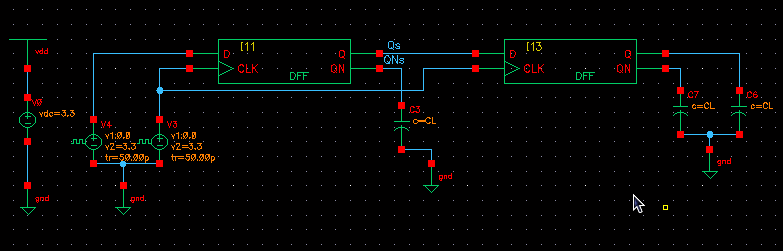
\includegraphics[width=0.45\textwidth]{Figures/DFFTestSchem.png}
\caption{DFF Test Circuit Schematic.}
\label {fig:DFFTestSchem}
\end{figure}

\section{Duel Edge Triggered Flip Flop}

\begin{figure}[h]  
\centering
   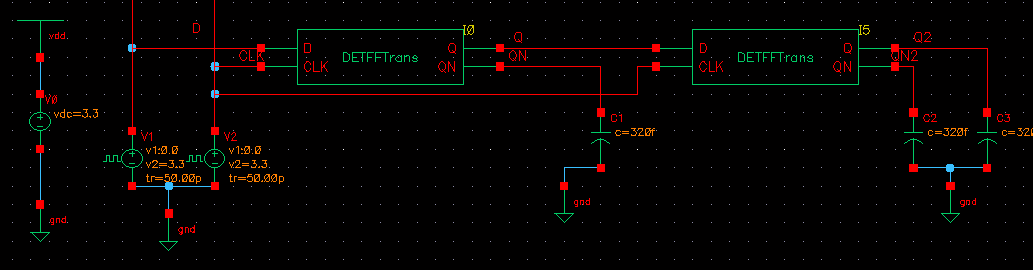
\includegraphics[width=0.45\textwidth]{Figures/DETFFTestSchem.png}
\caption{DETFF Test Circuit Schematic.}
\label {fig:DETFFTestSchem}
\end{figure}

\section{C Element}

\section{Dual Rail AND}

TEST CIRCUIT

\begin{figure}[h]  
\centering
   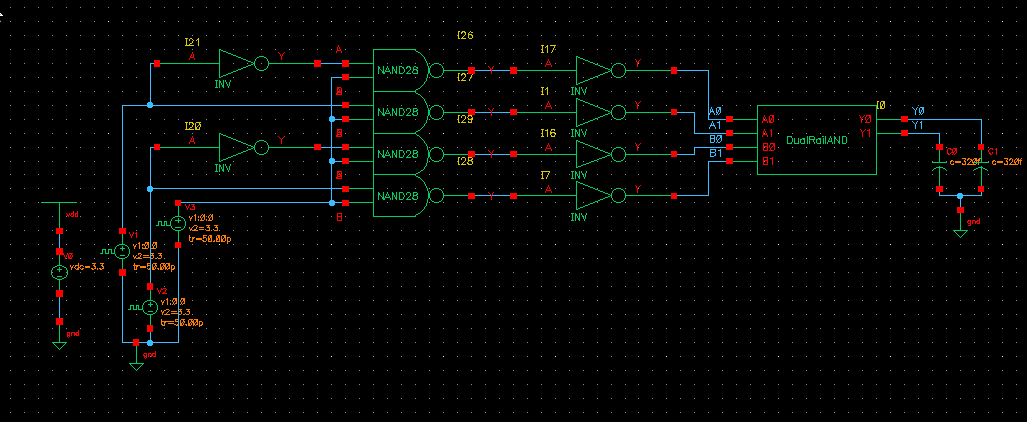
\includegraphics[width=0.45\textwidth]{Figures/DualRailANDTestSchem.png}
\caption{Dual Rail AND Test Schematic.}
\label {fig:DualRailANDTestSchem}
\end{figure}

FUNCTIONALITY TESTING 

\begin{figure}[h]  
\centering
   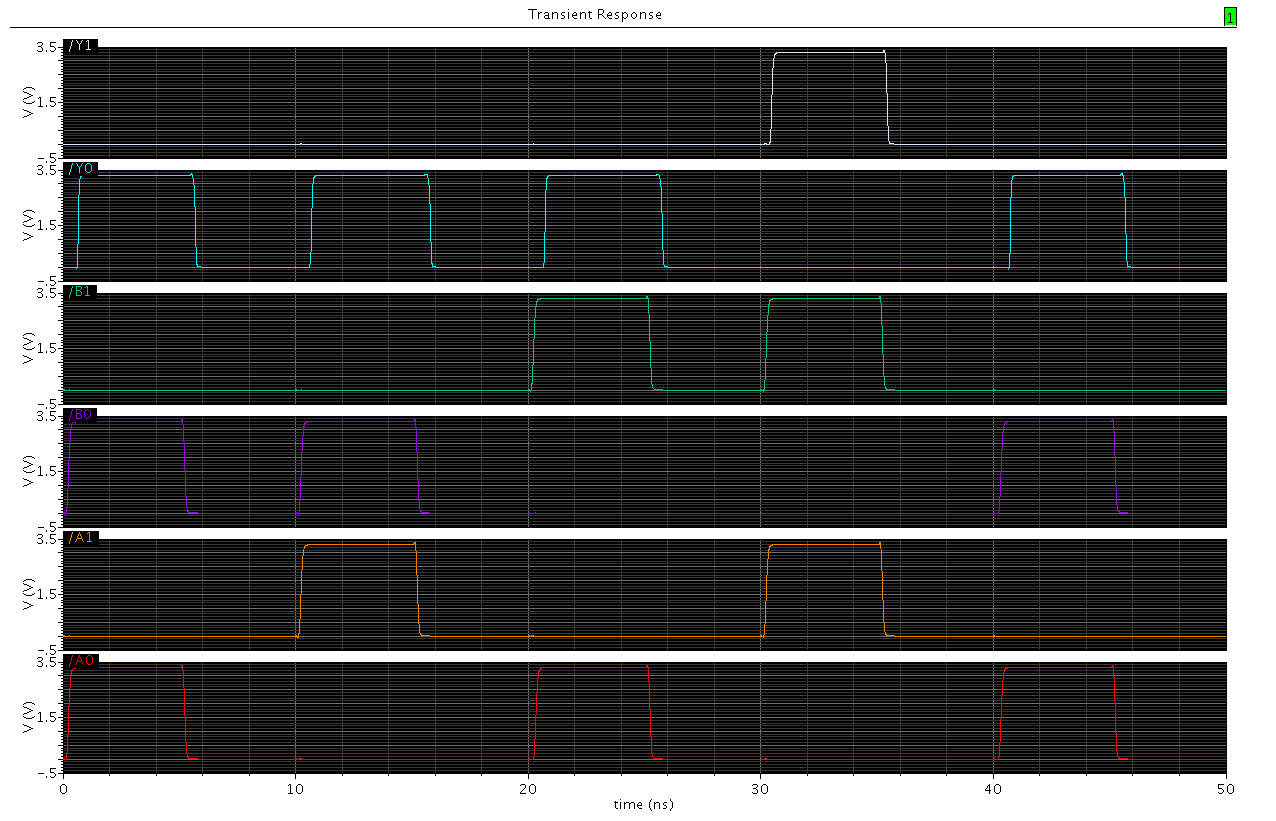
\includegraphics[width=0.45\textwidth]{Figures/DualAndCorrectOperation.png}
\caption{Dual Rail AND Simulation showing correct operation.}
\label {fig:DualAndCorrectOperation}
\end{figure}

SPEED TESTING

LAYOUT VS SCHEMATIC 

ERRONIOUS BEHAVIOUR







\section{1-bit Subtractor}

\section{2-to-1 Multiplexor}

\section{Mutex Element}

\chapter{Impact of Variablility}


\section{NAND}

\section{NOR2}

\section{XOR2}

\section{DFF}

VDD

TEMP


\section{Duel Edge Triggered Flip Flop}

VDD

TEMP

\section{C Element}

\section{Dual Rail AND}

\section{1-bit Subtractor}

\section{2-to-1 Multiplexor}

\section{Mutex Element}

\chapter{Conclusions}




%\addcontentsline{toc}{chapter}{References}
\bibliographystyle{IEEEtran}
\bibliography{Special/First_References}
%\end{document}
%% ----------------------------------------------------------------


%\appendix
%\appendixpage
%\addappheadtotoc
%%% ----------------------------------------------------------------
%% AppendixA.tex
%% ---------------------------------------------------------------- 


%\chapter{Something} \label{Chapter:Something}
\section{Statement of Contribution} \label{Section:Contribution}

Tables \ref{tab:jobs} and \ref{tab:jobs2} below detail the contributions of team members to the project.  While Ken Payne served as Team lead, Xuan Ban and Arinze Ekwosimba worked under his able leadership to ensure the project was delivered as required.  All members did significant research and contributed to the report writing as well.  The relative contribution of all authors is approximately equal.

\begin{table}
\begin{center}
\renewcommand{\arraystretch}{1.3}
\setlength{\tabcolsep}{7pt}
\begin{tabular}{ll}
\hline
\textbf{Group Member} & \textbf{Writing Task}\\
\hline
Arinze Ekwosimba & General editing of report, Wrote Abstract and Section Two (BT). \\
Kenneth Payne & Team Lead, wrote Introduction, Section One and Section Two (Intel) \\
Xuan Ban & Wrote Section Two (Nokia), Conclusion and Additional Notes \\
\hline
\end{tabular}
\caption{Report writing task allocation}
\label{tab:jobs}%
\end{center}
\end{table}

\begin{table}
\begin{center}
\renewcommand{\arraystretch}{1.3}
\setlength{\tabcolsep}{7pt}
\begin{tabular}{ll}
\hline
\textbf{Group Member} & \textbf{Research Task}\\
\hline
Arinze Ekwosimba & Gathered evidence on BT and Intel \\
Kenneth Payne & Gathered evidence on Intel \\
Xuan Ban & Gathered evidence on Nokia \\
\hline
\end{tabular}
\caption{Evidence Collation task allocation}
\label{tab:jobs2}%
\end{center}
\end{table}
%%% ----------------------------------------------------------------
%% AppendixB.tex
%% ---------------------------------------------------------------- 


%\chapter{Something} \label{Chapter:Something}
\section{Meeting Minutes} \label{Section:Minutes}

	\begin{figure}[ht!]
		\centering
		\includegraphics[width = 0.9\textwidth]{Figures/Minutes_1}
		\caption[Minutes I]{Minutes of the first group meeting}
		\label {fig:minutes:one}
	\end{figure}
	
		\begin{figure}[ht!]
		\centering
		\includegraphics[width = 0.9\textwidth]{Figures/Minutes_2}
		\caption[Minutes II]{Minutes of the second group meeting}
		\label {fig:minutes:two}
	\end{figure}
	
		\begin{figure}[ht!]
		\centering
		\includegraphics[width = 0.9\textwidth]{Figures/Minutes_3}
		\caption[Minutes III]{Minutes of the third group meeting}
		\label {fig:minutes:three}
	\end{figure}
%%% ----------------------------------------------------------------
%% AppendixC.tex
%% ---------------------------------------------------------------- 


%\chapter{Something} \label{Chapter:Something}
\section{Additional Notes} \label{Section:Notes}


	\begin{figure}[ht!]
		\centering
		%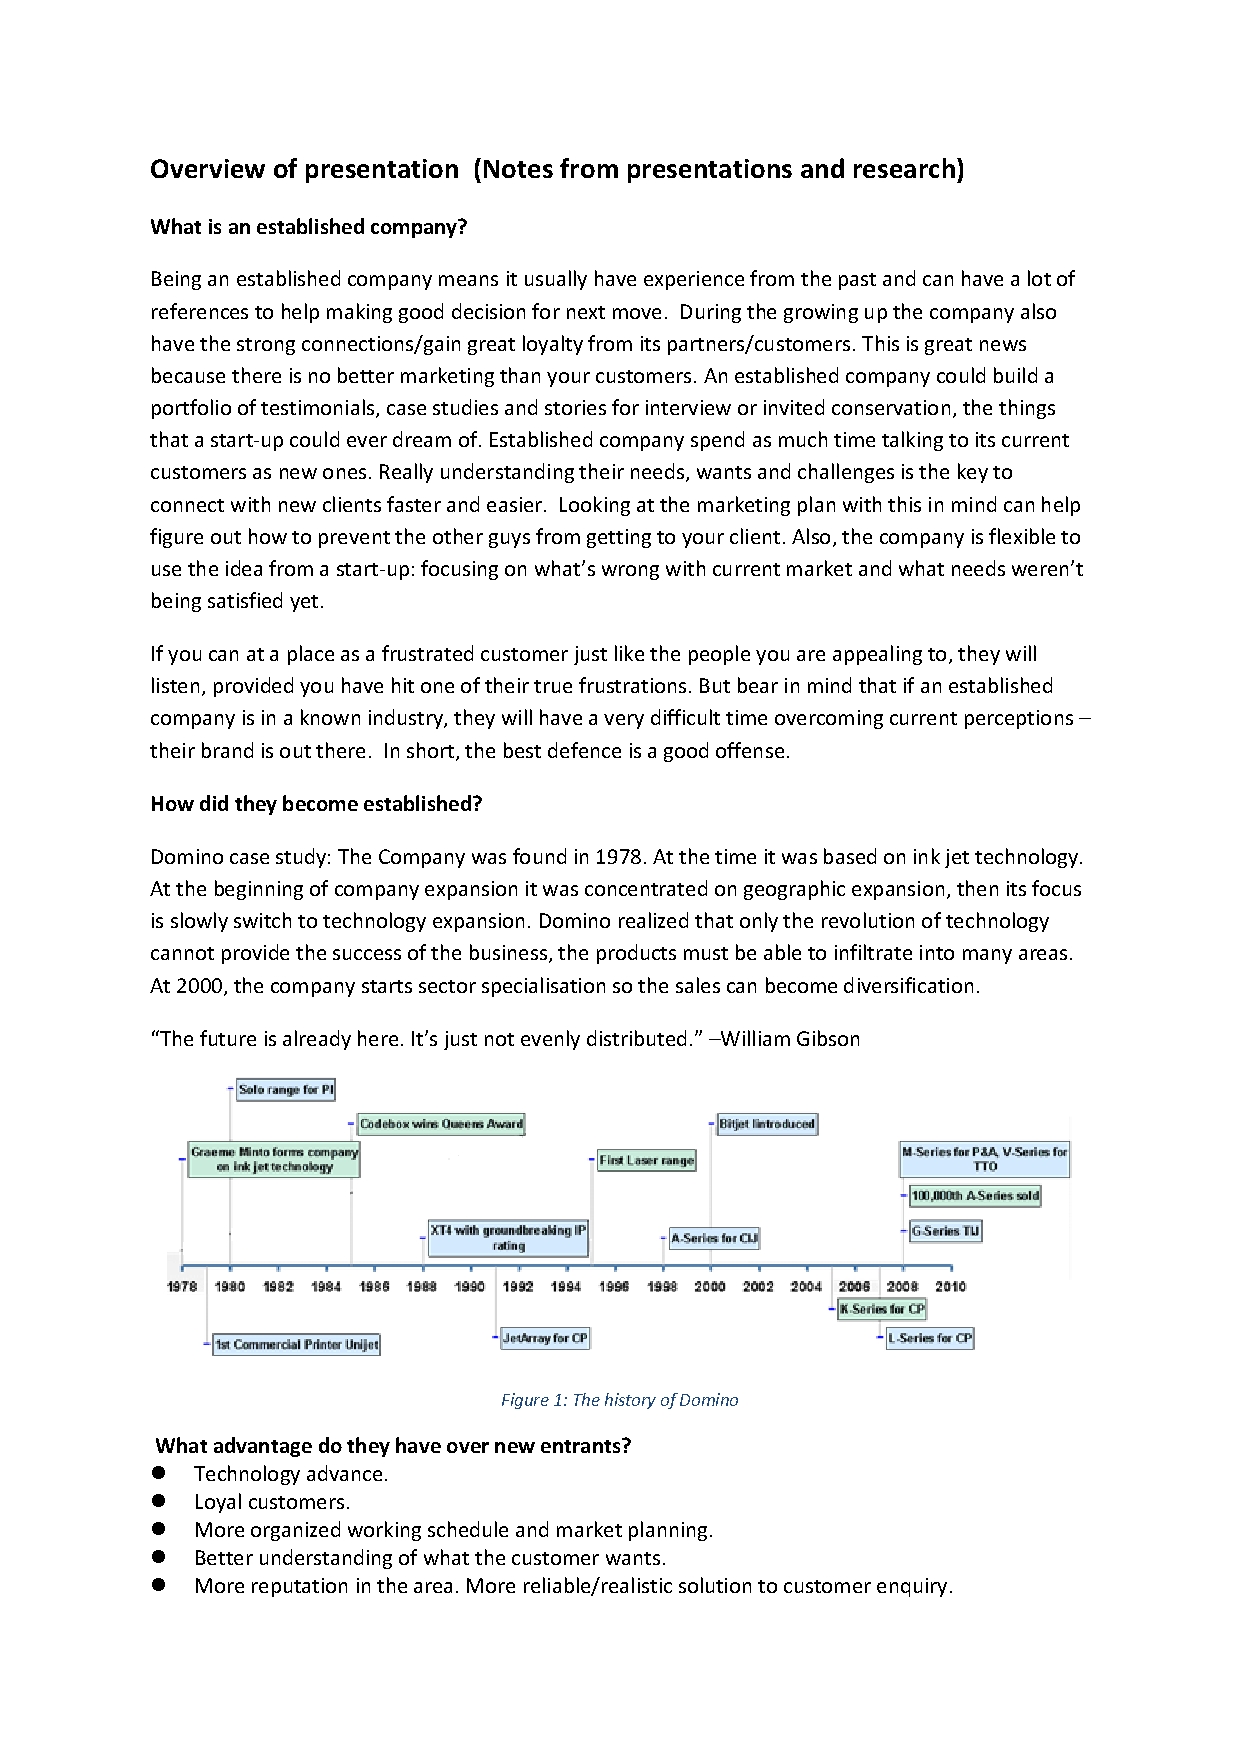
\includegraphics[width = 0.9\textwidth]{Figures/Overview_of_presentations}
		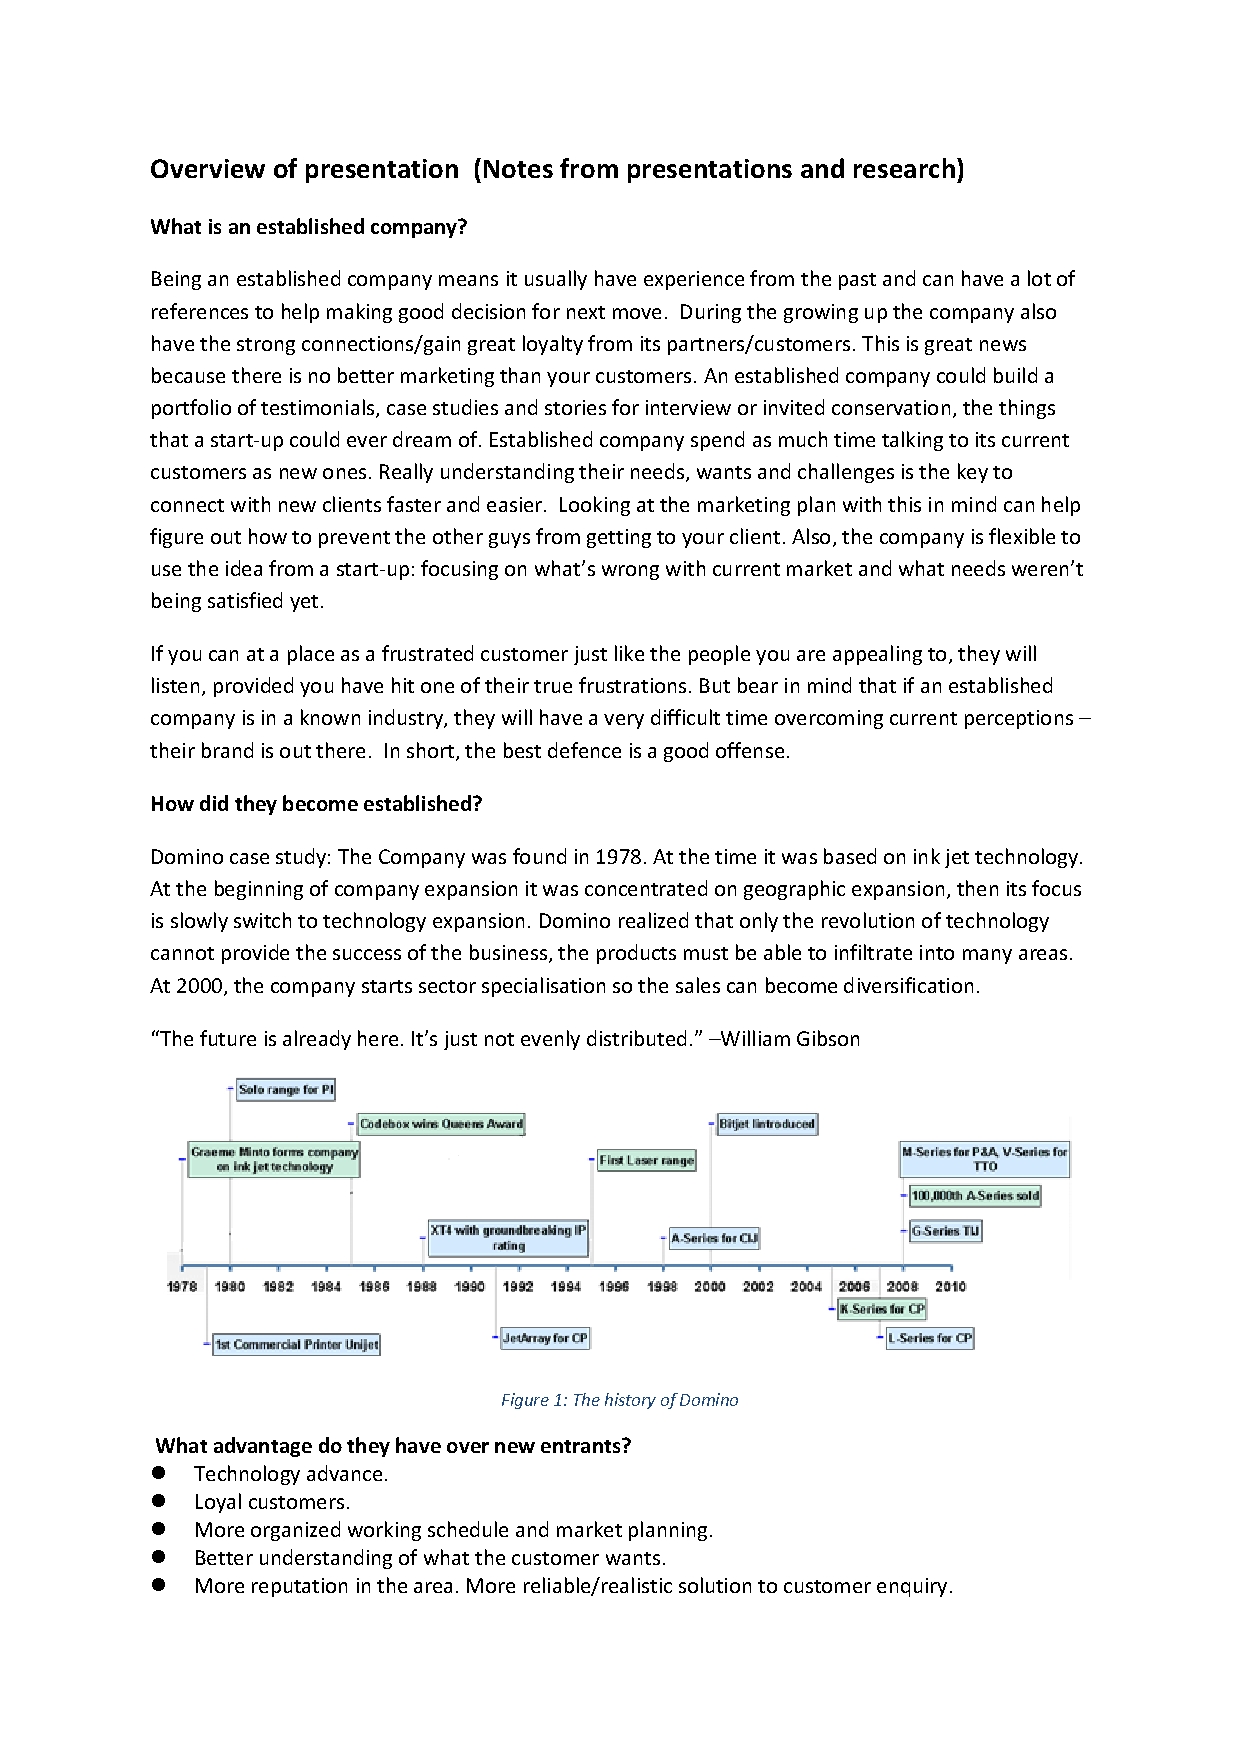
\includegraphics[width = 0.9\textwidth, page=1]{Figures/Overview_of_presentations}		
		%\caption[Additional Notes]{Notes taken for given presentations and independent research}
		\label {fig:additional:notes1}
	\end{figure}
	
		\begin{figure}[ht!]
		\centering
		%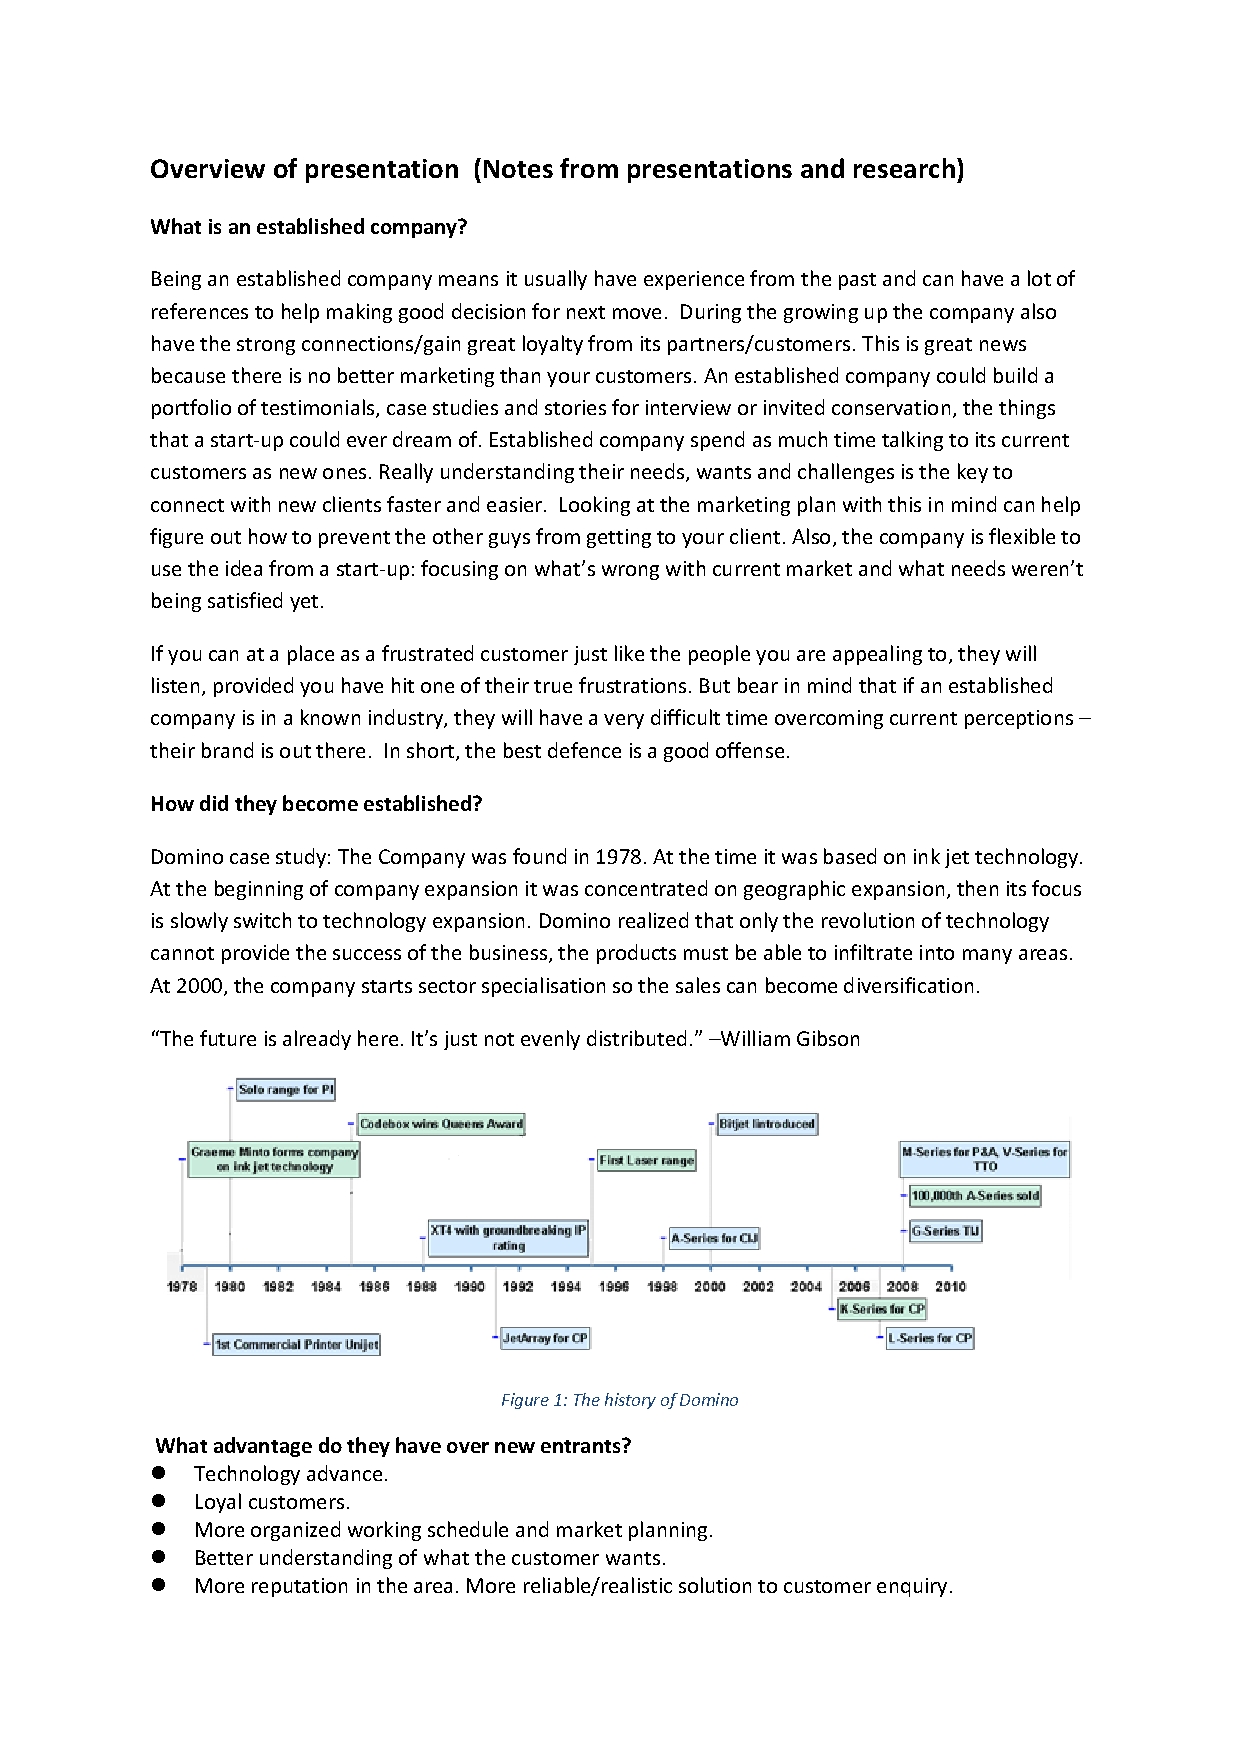
\includegraphics[width = 0.9\textwidth]{Figures/Overview_of_presentations}
		\includegraphics[width = \textwidth, page=2]{Figures/Overview_of_presentations}		
		%\caption[Additional Notes]{Notes taken for given presentations and independent research}
		\label {fig:additional:notes2}
	\end{figure}
	
		\begin{figure}[ht!]
		\centering
		%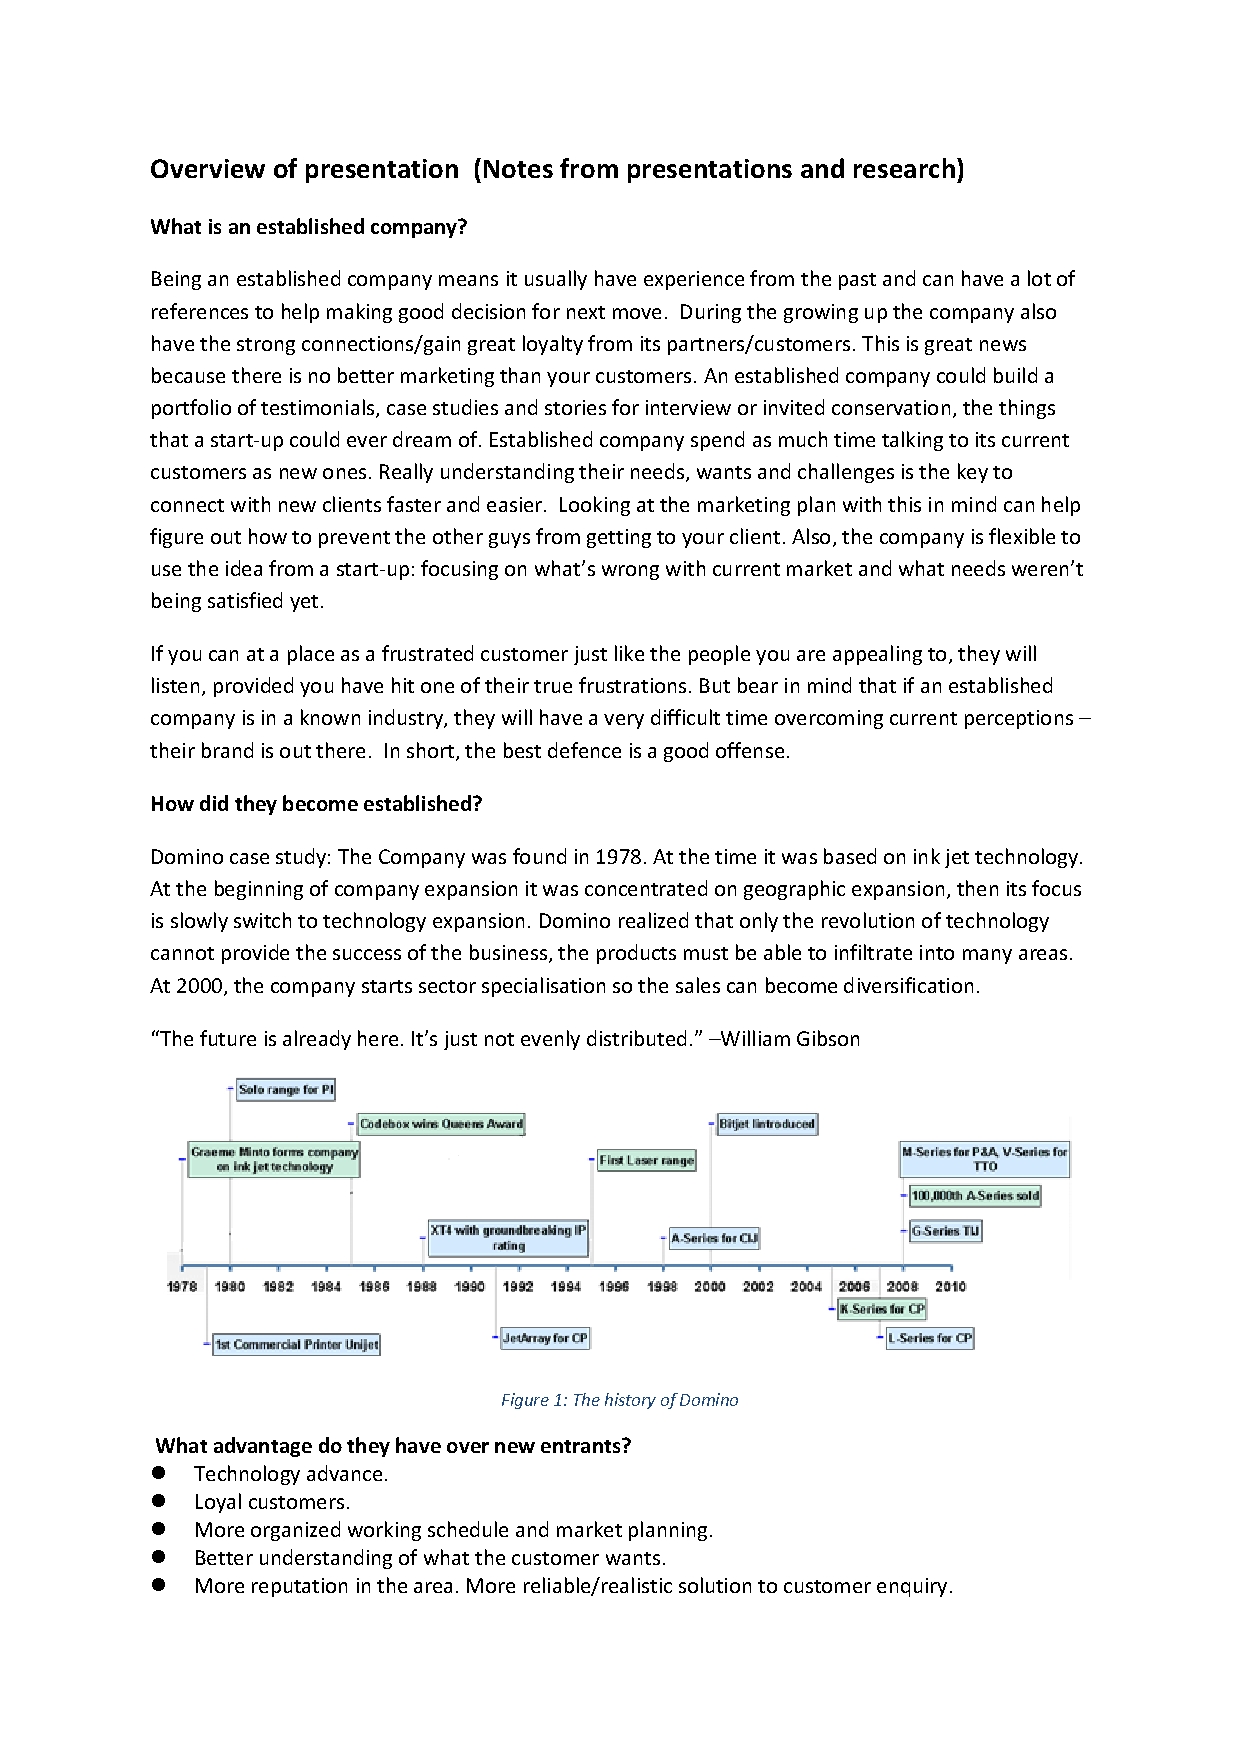
\includegraphics[width = 0.9\textwidth]{Figures/Overview_of_presentations}
		\includegraphics[width = \textwidth, page=3]{Figures/Overview_of_presentations}		
		%\caption[Additional Notes]{Notes taken for given presentations and independent research}
		\label {fig:additional:notes3}
	\end{figure}
	
		\begin{figure}[ht!]
		\centering
		%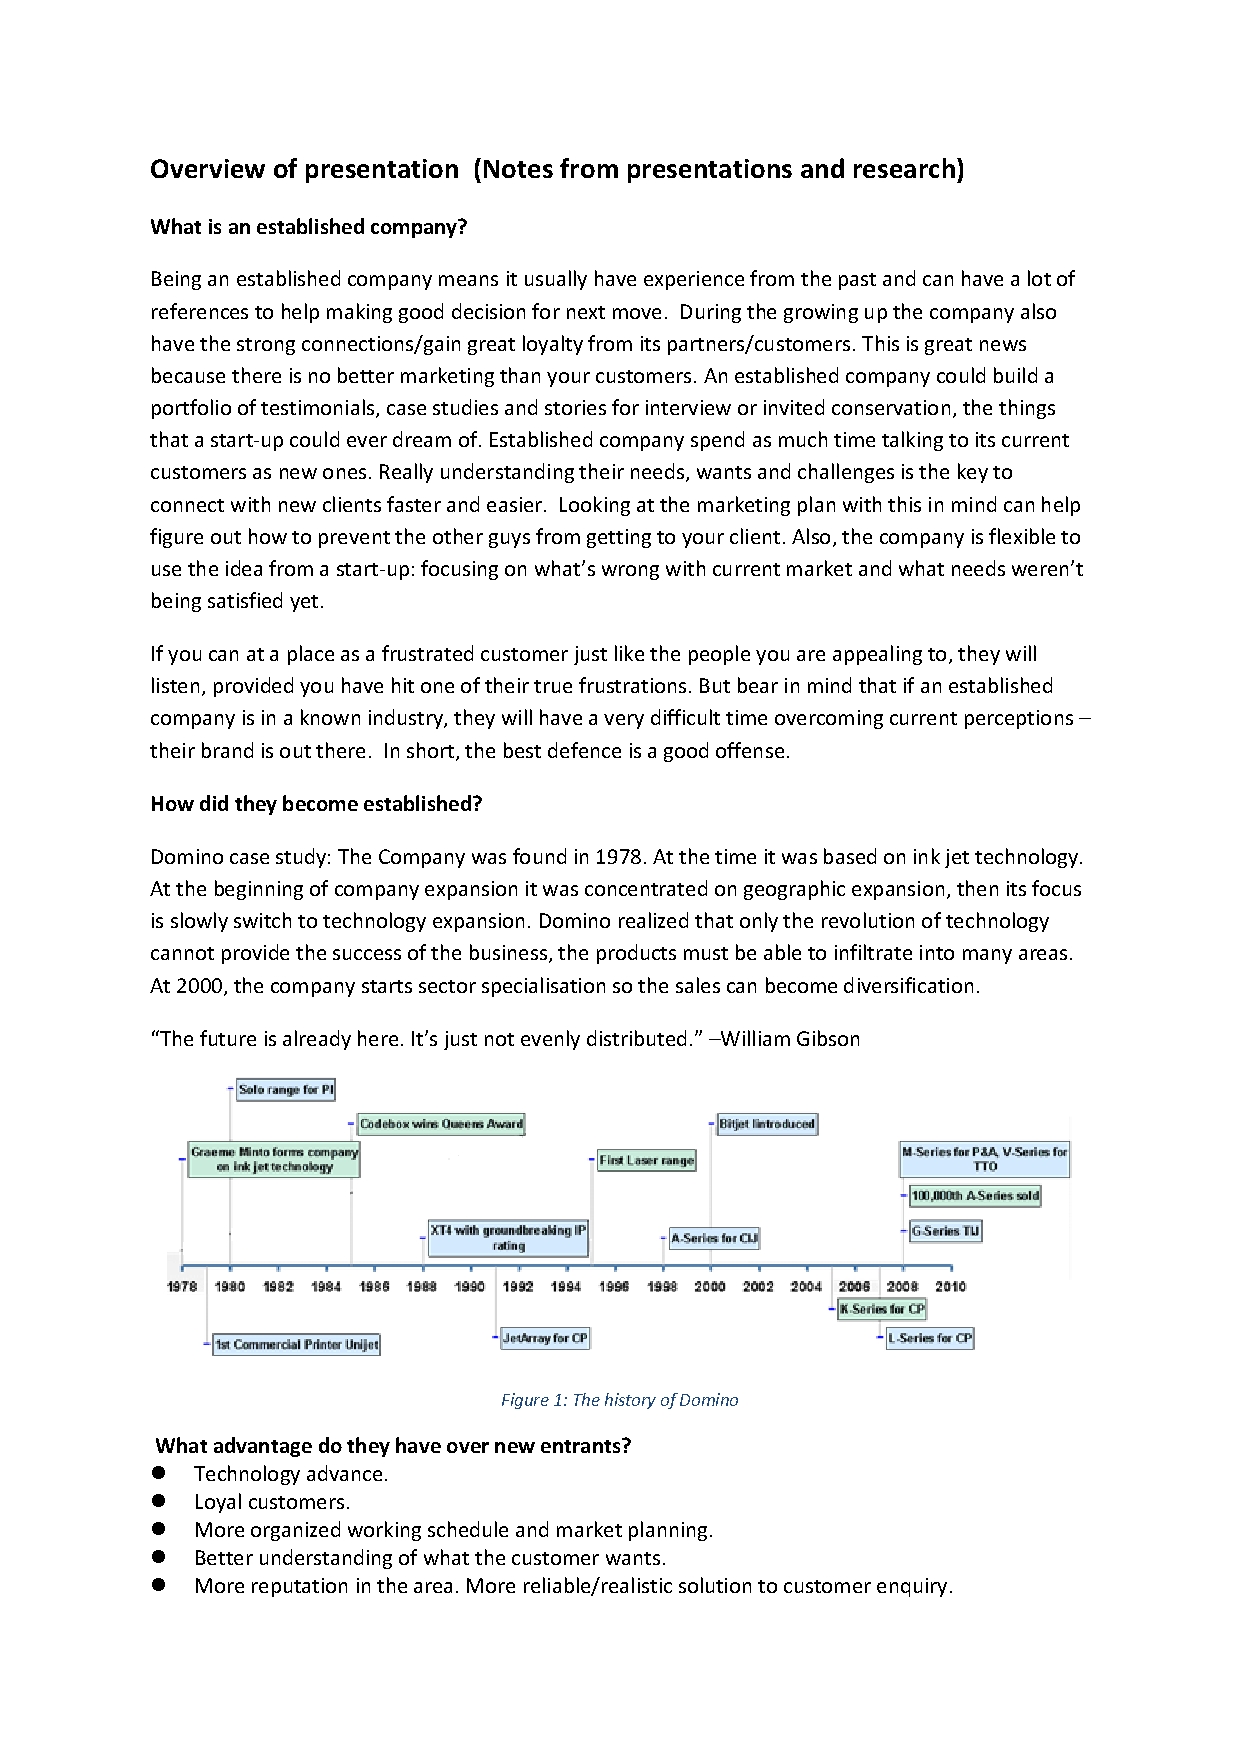
\includegraphics[width = 0.9\textwidth]{Figures/Overview_of_presentations}
		\includegraphics[width = \textwidth, page=4]{Figures/Overview_of_presentations}		
		%\caption[Additional Notes]{Notes taken for given presentations and independent research}
		\label {fig:additional:notes4}
	\end{figure}
	
		\begin{figure}[ht!]
		\centering
		%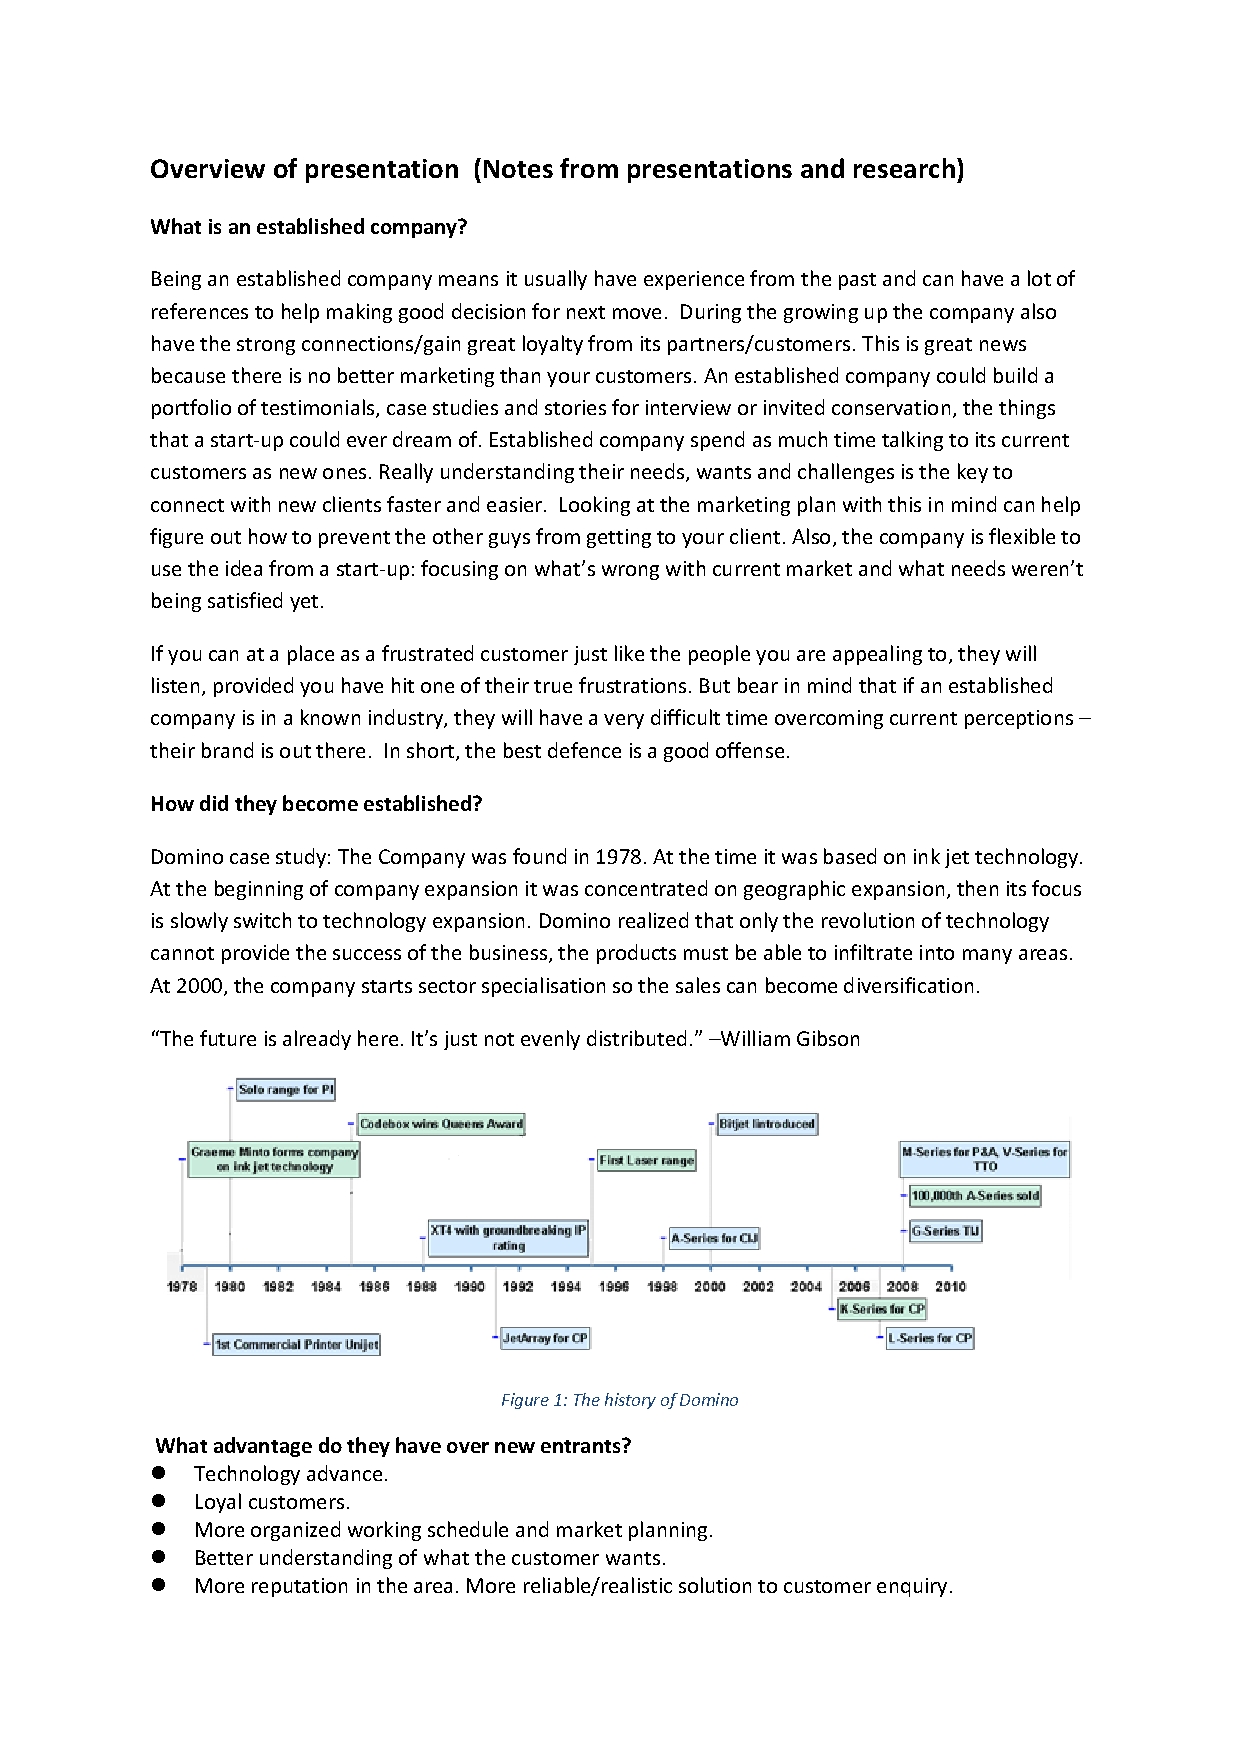
\includegraphics[width = 0.9\textwidth]{Figures/Overview_of_presentations}
		\includegraphics[width = \textwidth, page=5]{Figures/Overview_of_presentations}		
		\caption[Additional Notes]{Notes taken for given presentations and independent research}
		\label {fig:additional:notes5}
	\end{figure}
%\include{Appendices/AppendixD}
%\include{Appendices/AppendixE}

\end{document}
